% -------------------------------------------------------
% This plot is from DefElement (https://defelement.com)
% and is available under a Creative Commons Attribution
% 4.0 International (CC BY 4.0) license:
% https://creativecommons.org/licenses/by/4.0/
% -------------------------------------------------------
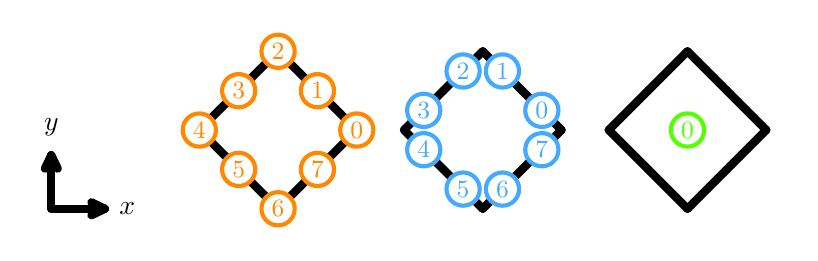
\begin{tikzpicture}[x=0.2mm,y=0.2mm]
\definecolor{color1}{HTML}{FF8800}
\definecolor{color2}{HTML}{44AAFF}
\definecolor{color3}{HTML}{55FF00}
\clip (0,0) rectangle (484,130);
\draw[black,line width=3pt,line cap=round](15.0,15.0) -- (49.0,15.0);
\draw[black,line width=3pt,line cap=round](40.5,10.92) -- (49.0,15.0);
\draw[black,line width=3pt,line cap=round](40.5,19.08) -- (49.0,15.0);
\draw[black,line width=3pt,line cap=round](15.0,15.0) -- (15.0,49.0);
\draw[black,line width=3pt,line cap=round](19.08,40.5) -- (15.0,49.0);
\draw[black,line width=3pt,line cap=round](10.92,40.5) -- (15.0,49.0);
\draw[black,line width=3pt,line cap=round](209.0,65.0) -- (184.0,90.0);
\draw[black,line width=3pt,line cap=round](184.0,90.0) -- (159.0,115.0);
\draw[black,line width=3pt,line cap=round](159.0,115.0) -- (134.0,90.0);
\draw[black,line width=3pt,line cap=round](134.0,90.0) -- (109.0,65.0);
\draw[black,line width=3pt,line cap=round](109.0,65.0) -- (134.0,40.0);
\draw[black,line width=3pt,line cap=round](134.0,40.0) -- (159.0,15.0);
\draw[black,line width=3pt,line cap=round](159.0,15.0) -- (184.0,40.0);
\draw[black,line width=3pt,line cap=round](184.0,40.0) -- (209.0,65.0);
\draw[black,line width=3pt,line cap=round](339.0,65.0) -- (314.0,90.0);
\draw[black,line width=3pt,line cap=round](314.0,90.0) -- (289.0,115.0);
\draw[black,line width=3pt,line cap=round](289.0,115.0) -- (264.0,90.0);
\draw[black,line width=3pt,line cap=round](264.0,90.0) -- (239.0,65.0);
\draw[black,line width=3pt,line cap=round](239.0,65.0) -- (264.0,40.0);
\draw[black,line width=3pt,line cap=round](264.0,40.0) -- (289.0,15.0);
\draw[black,line width=3pt,line cap=round](289.0,15.0) -- (314.0,40.0);
\draw[black,line width=3pt,line cap=round](314.0,40.0) -- (339.0,65.0);
\draw[black,line width=3pt,line cap=round](469.0,65.0) -- (444.0,90.0);
\draw[black,line width=3pt,line cap=round](444.0,90.0) -- (419.0,115.0);
\draw[black,line width=3pt,line cap=round](419.0,115.0) -- (394.0,90.0);
\draw[black,line width=3pt,line cap=round](394.0,90.0) -- (369.0,65.0);
\draw[black,line width=3pt,line cap=round](369.0,65.0) -- (394.0,40.0);
\draw[black,line width=3pt,line cap=round](394.0,40.0) -- (419.0,15.0);
\draw[black,line width=3pt,line cap=round](419.0,15.0) -- (444.0,40.0);
\draw[black,line width=3pt,line cap=round](444.0,40.0) -- (469.0,65.0);
\node[anchor=west] at (52.0,15.0) {$x$};
\node[anchor=south] at (15.0,55.0) {$y$};
\draw[color1,fill=white,line width=1.5pt] (209.0,65.0)circle (6pt);
\node[anchor=center] at (209.0,65.0) {\small\color{color1}0};
\draw[color1,fill=white,line width=1.5pt] (184.0,90.0)circle (6pt);
\node[anchor=center] at (184.0,90.0) {\small\color{color1}1};
\draw[color1,fill=white,line width=1.5pt] (159.0,115.0)circle (6pt);
\node[anchor=center] at (159.0,115.0) {\small\color{color1}2};
\draw[color1,fill=white,line width=1.5pt] (134.0,90.0)circle (6pt);
\node[anchor=center] at (134.0,90.0) {\small\color{color1}3};
\draw[color1,fill=white,line width=1.5pt] (109.0,65.0)circle (6pt);
\node[anchor=center] at (109.0,65.0) {\small\color{color1}4};
\draw[color1,fill=white,line width=1.5pt] (134.0,40.0)circle (6pt);
\node[anchor=center] at (134.0,40.0) {\small\color{color1}5};
\draw[color1,fill=white,line width=1.5pt] (159.0,15.0)circle (6pt);
\node[anchor=center] at (159.0,15.0) {\small\color{color1}6};
\draw[color1,fill=white,line width=1.5pt] (184.0,40.0)circle (6pt);
\node[anchor=center] at (184.0,40.0) {\small\color{color1}7};
\draw[color2,fill=white,line width=1.5pt] (326.5,77.5)circle (6pt);
\node[anchor=center] at (326.5,77.5) {\small\color{color2}0};
\draw[color2,fill=white,line width=1.5pt] (301.5,102.5)circle (6pt);
\node[anchor=center] at (301.5,102.5) {\small\color{color2}1};
\draw[color2,fill=white,line width=1.5pt] (276.5,102.5)circle (6pt);
\node[anchor=center] at (276.5,102.5) {\small\color{color2}2};
\draw[color2,fill=white,line width=1.5pt] (251.5,77.5)circle (6pt);
\node[anchor=center] at (251.5,77.5) {\small\color{color2}3};
\draw[color2,fill=white,line width=1.5pt] (251.5,52.5)circle (6pt);
\node[anchor=center] at (251.5,52.5) {\small\color{color2}4};
\draw[color2,fill=white,line width=1.5pt] (276.5,27.5)circle (6pt);
\node[anchor=center] at (276.5,27.5) {\small\color{color2}5};
\draw[color2,fill=white,line width=1.5pt] (301.5,27.5)circle (6pt);
\node[anchor=center] at (301.5,27.5) {\small\color{color2}6};
\draw[color2,fill=white,line width=1.5pt] (326.5,52.5)circle (6pt);
\node[anchor=center] at (326.5,52.5) {\small\color{color2}7};
\draw[color3,fill=white,line width=1.5pt] (419.0,65.0)circle (6pt);
\node[anchor=center] at (419.0,65.0) {\small\color{color3}0};
\end{tikzpicture}